\documentclass{beamer}
\title{Klemens z Ochrydy}
\author{Adam Stepanczuk}
\date{\today}
\usepackage{amsfonts}
\usepackage{polski}
\usepackage[utf8]{inputenc}
\usepackage{graphicx}

\usetheme{CambridgeUs}
\usecolortheme{seahorse}
\begin{document}
\frame{\titlepage}

\section{Klemens-wstęp}
\begin{frame}
\frametitle{Kim był Klemens z Ochrydy}
Bułgar, Macedończyk, uczeń świętych: Cyryla i Metodego, biskup Drembicy i Belitsy, arcybiskup Ochrydy, pierwszy biskup i apostoł Bułgarii, współtwórca rytu słowiańskiego, święty prawosławny i katolicki.
\begin{figure}
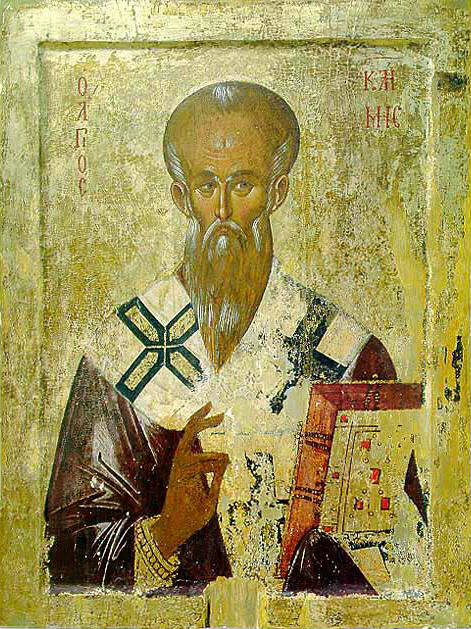
\includegraphics[scale=0.25]{Climent_of_Ohrid.jpg}
\end{figure}
\end{frame}

\section{Nauczyciele Klemensa}
\begin{frame}{Nauczyciele Klemensa z Ochrydy}
Święty Cyryl, właściwie Konstantyn, (ur. ok. 827 w Tesalonice, zm. 14 lutego 869) i Święty Metody, właśc. Michał, (ur. ok. 815, zm. 6 kwietnia 885), Bracia Sołuńscy, misjonarze. Prowadzili w IX wieku misje chrystianizacyjne, m.in. na ziemiach zamieszkanych przez Słowian. Twórcy rytu słowiańskiego, święci Kościoła katolickiego i prawosławnego nazywani apostołami Słowian  i apostołami Bułgarii.
\begin{figure}
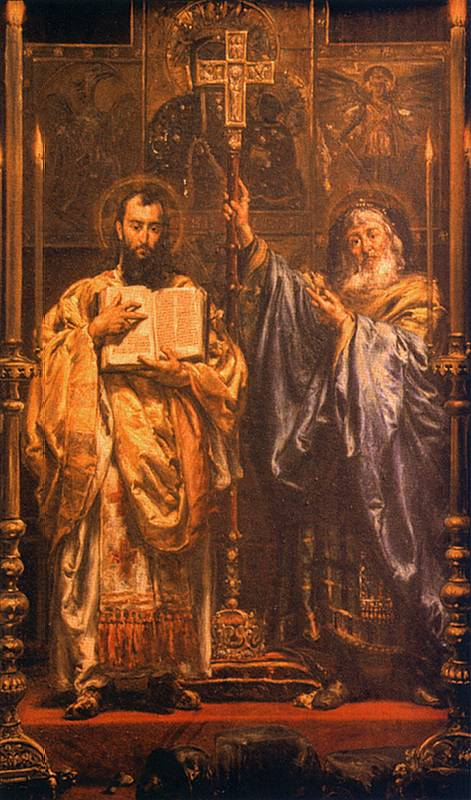
\includegraphics[scale=0.6]{Cyril_and_Methodius.jpg}
\end{figure}
\end{frame}

\section{Żywot świętego}
\begin{frame}
\frametitle{Żywot świętego}
Data urodzenia Klemensa nie jest znana. Był najprawdopodobniej Słowianinem pochodzącym z Macedonii. Bardzo wcześnie został uczniem Konstantyna i Metodego. Miał im towarzyszyć już w misji chazarskiej (860-861), w czasie której na cześć odnalezionych przez Metodego w Chersonezie relikwii świętego Klemensa papieża, nadano mu imię Klemens
\end{frame}

\begin{frame}{Żywot świętego cd.}
W 885 roku biskup Metody zmarł na Morawach. Jako swego następcę wyznaczył Gorazda. Ten nie zdołał jednak sprostać opozycji duchownych łacińskich wspieranych przez księcia morawskiego Świętopełka. Przywódcy słowiańskiego kościoła na Morawach: Gorazd, Klemens, Naum, Angelary, Laurencjusz i Sawa zostali uwięzieni i poddani torturom. Klemens, Naum i Angelary, wygnani z Moraw zostali serdecznie przyjęci przez namiestnika Borysa w Belgradzie. Książę Borys udzielił im w Plisce gościny w domach swych dostojników, umieszczając Klemensa i Nauma u sampsesa Eschacza, a Angelarego u Czesława.
\end{frame}

\begin{frame}{Żywot świętego cd.}
Na objętym przez siebie terenie Klemens rozwinął szeroko zakrojoną działalność apostolską. Stale podróżując, nauczając i studiując, wykształcił około trzech i pół tysiąca kapłanów. Skupił wokół siebie krąg wykształconych uczniów, którzy wspierali go w pracy kościelnej i oświatowo-literackiej, a potem podjęli jego pracę. W 893 roku został powołany przez nowego władcę Symeona na biskupa Drewenicy---Welicy położonej na północ od Ochrydu.
\end{frame}

\section{Spuścizna}
\begin{frame}{Pisma}
Klemens kontynuował pracę przekładową Cyryla i Metodego, tłumacząc z greckiego te części Pisma Świętego i liturgii bizantyńskiej, których oni nie zdążyli oddać po słowiańsku. Pozostawił po sobie liczne kazania i homilie oraz eulogie. Zachowało się około 50 kazań i eulogii. Wśród dzieł przypisywanych Klemensowi w oparciu o analizę językową wymienia się: Legendy pannońskie, Ordo Confessionis z Euchologium synajskiego i pewne części głagolickich fragmentów Cloza. Przypuszcza się także, że tzw. Zabytki fryzyńskie mają związek z twórczością Klemensa.
\end{frame}

\begin{frame}{Pisma cd.}
Pisma Klemensa stały się po jego śmierci tak popularne i cieszyły się tak wielkim autorytetem, że wiele z nich kopiści zaczęli przypisywać Janowi Chryzostomowi. Sława ich rozprzestrzeniła się w całym świecie słowiańskim. Po chrzcie Rusi w 988 roku, wiele pism Klemensa trafiło na Ruś. Po upadku państwa bułgarskiego w ciągu XI i XII wieku dorobek Klemensa został prawie doszczętnie zniszczony przez duchowieństwo greckie, które tępiło piśmiennictwo słowiańskie zarzucając mu herezję i uleganie wpływom bogomilskim
\end{frame}

\begin{frame}{Klemens a głagolica}
Dyskutowany jest stosunek Klemensa do głagolicy alfabetu utworzonego przez Konstantyna. Według części uczonych Klemens pisał wyłącznie w głagolicy i dlatego nie pozostał w Presławiu. Istnieje nawet przypuszczenie, że nie mogąc go nakłonić do używania cyrylicy władca bułgarski celowo wysłał go w najdalszy zakątek państwa. Istnieją i sądy przeciwne, które twierdzą, że Klemens zastawszy po ucieczce z Moraw w Presławiu cyrylicę, sam zaczął stopniowo zastępować nią teksty zapisane głagolicą.
\end{frame}

\section{Kult}
\begin{frame}{Kult}
W dowód wielkich zasług Bułgarska Cerkiew Prawosławna nadała świętemu tytuł równego apostołom, a uniwersytet w Sofii nosi jego imię. Jest jednym z największych świętych na Bałkanach.

Cerkiew prawosławna wspomina świętego dwukrotnie:
\begin{itemize}
\item<2-4> 27 lipca/9 sierpnia, tj. 9 sierpnia według kalendarza gregoriańskiego (Sobór bułgarskich oświecicieli)
\item<3-4> 25 listopada/8 grudnia tj. 8 grudnia (razem ze św. Klemensem, papieżem).
\item<4> W Kościele katolickim wspominany jest w grupie Siedmiu Apostołów Bułgarii dawniej 17 lipca (dzień śmierci), a w nowym Martyrologium Rzymskim 22 listopada.
\end{itemize}
\end{frame}

\end{document}
